% Chapter Template

% Main chapter title
\chapter{Results}

% Short version of the title for the header
\chaptermark{Results}

% Chapter Label
\label{chap:results}

This chapter presents the experimental results of our tokenizer adaptation method. We first report quantitative evaluations, covering initialization strategies, benchmark accuracy, tokenization efficiency, rank distributions, and retention of source language effectiveness.
These findings are later complemented by a qualitative evaluation of model completions and, finally, the chapter concludes with a discussion that synthesizes the implications of both quantitative and qualitative results, while noting encountered limitations.


\section{Quantitative Results}

Throughout this section, we provide evidence to support our conclusions on the effects of vocabulary expansion and embedding initialization. Each subsection reports results with a reflection on their meaning for the research questions guiding this work, as proposed in Section~\ref{sec:objectives}


\subsection{Embedding Initialization Strategies}
\label{subsec:results}

By focusing on embedding initialization strategies, we directly explore our RQ4, which concerns the impact of embedding initialization strategies on the stability and usefulness of adapted vocabularies.

\begin{table}[ht]
    \centering
    \begin{tabular}{l c}
        \toprule
        Initialization Method & Number of Wins \\
        \midrule
        Random Initialization & 36 \\
        Mean Vector Initialization & 39 \\
        Weighted Drop ($\alpha=0.5$) & 26 \\
        Weighted Drop ($\alpha=1.0$) & 37 \\
        Weighted Drop ($\alpha=1.5$) & 47 \\
        Weighted Drop ($\alpha=2.0$) & 53 \\
        Weighted Drop ($\alpha=2.5$) & 81 \\
        Weighted Drop ($\alpha=3.0$) & 89 \\
        Weighted Drop ($\alpha=3.5$) & 79 \\
        Weighted Drop ($\alpha=4.0$) & 99 \\
        Weighted Drop ($\alpha=4.5$) & 126 \\
        Weighted Drop ($\alpha=5.0$) & 127 \\
        \bottomrule
    \end{tabular}
    \caption{Frequency of best prediction (lowest rank) across 1,000 sampled lines for each initialization strategy.}
    \label{tab:embed_init_results}
\end{table}

Using the methodology described in Section~\ref{sec:init_methodology}, we compared initialization strategies by counting, for each method, how often it produced the best prediction (lowest score) for a new token across 1,000 sampled lines. This metric reflects the model’s ability to correctly predict unseen tokens given partial context.

Table~\ref{tab:embed_init_results} presents results across models. Random initialization often led to unstable behavior, while both mean and position-weighted approaches were more reliable. Among these, the position-weighted strategy produced embeddings that better reflected token context, and so it was selected for the remaining experiments.

These results form the empirical foundation for discussing RQ4. A more comprehensive evaluation of their significance will follow later.





\subsection{Benchmark Accuracy}
In this section we make use of the benchmarks introduced in Section~\ref{sec:ptpt-benchmarks-intro}, so as to reinforce our strategy. Additionally, we explore questions \textbf{RQ1}, which focuses on the effectiveness of the adapted model in the target language.

The main benchmarks we focus on are: \textit{CalamePT}, built to evaluate comprehension on Portuguese text by providing our models with incomplete phrases where the last word is easily obtainable through the context; \textit{extraGLUE}, built to capture data on reasoning and text comprehension of a model, by providing it with questions where the answer does not directly emerge from it; and \textit{SuperGLUE}, which is the original English version of \textit{extraGLUE} making it useful for comparing a model’s Portuguese effectiveness with its English counterpart.

Since the benchmark evaluation was designed to test whether adapted vocabularies improve accuracy on downstream tasks, each baseline model was therefore compared with two variants: one containing only the new tokens, and another in which those tokens were also given lightweight embedding training (\S\ref{sec:embedding_finetune}).

The results, shown in Table~\ref{tab:benchmark-results}, cover three models of different sizes: \texttt{SmolLM2-135M}, \texttt{SmolLM3-3B}, and \texttt{Qwen2.5-1.5B-Instruct}.

\begin{table}[H]
\centering
\begin{tabular}{ccccc}
\hline
\textbf{New Tokens} & \textbf{Type} & \textbf{CalamePT} & \textbf{extraGLUE\footnote{\textit{extraGLUE} evaluated with task boolQ}} & \textbf{SuperGLUE\footnote{\textit{SuperGLUE} evaluated with task boolQ}} \\
\hline
\multicolumn{5}{c}{\textbf{Model:} \emph{HuggingFaceTB/SmolLM2-135M}} \\
 0     & Baseline      & 13.54 \% & 1.47 \% & 41.02 \% \\
 1000  & No Training   & 13.54 \% & 1.47 \% & - \\
 1000  & With Training & 13.54 \% & 1.47 \% & - \\
 5000  & No Training   & 13.54 \% & 1.51 \% & - \\
 5000  & With Training & 13.54 \% & 1.51 \% & - \\
 7500  & No Training   & 13.54 \% & 1.51 \% & - \\
 7500  & With Training & 13.54 \% & 1.51 \% & - \\
\hline
\multicolumn{5}{c}{\textbf{Model:} \emph{HuggingFaceTB/SmolLM3-3B}} \\
0     & Baseline      & 58.53 \% & 49.69 \% & 38.45 \% \\
1000  & No Training   & 58.53 \% & 49.69 \% & - \\
1000  & With Training & 58.53 \% & 49.69 \% & - \\
5000  & No Training   & 58.53 \% & 49.69 \% & - \\
5000  & With Training & 58.53 \% & 49.69 \% & - \\
7500  & No Training   & 58.53 \% & 49.69 \% & - \\
7500  & With Training & 58.53 \% & 49.69 \% & - \\
\hline
\multicolumn{5}{c}{\textbf{Model:} \emph{Qwen/Qwen2.5-1.5B-Instruct}} \\
0     & Baseline      & 49.61 \% & 40.24 \% & 60.88 \% \\
1000  & No Training   & 49.61 \% & 39.86 \% & - \\
1000  & With Training & 49.61 \% & 39.79 \% & - \\
5000  & No Training   & 49.61 \% & 40.28 \% & - \\
5000  & With Training & 49.61 \% & 40.21 \% & - \\
7500  & No Training   & 49.57 \% & 40.14 \% & - \\
7500  & With Training & 49.57 \% & 40.06 \% & - \\
\hline
\end{tabular}
\caption{Results on Portuguese Benchmarks (\emph{CalamePT} and \emph{extraGLUE})}
\label{tab:benchmark-results}
\end{table}

Overall, benchmark accuracy remains stable across most configurations. Minor fluctuations (≤0.5\%) suggest that vocabulary expansion has little effect on high-level reasoning (\emph{extraGLUE}) or text completion (CalamePT) without more extensive training. Unsurprisingly, model effectiveness for English remained superior to that of Portuguese.



\subsection{Generation Efficiency}
\label{sec:gen_efficiency}

Whereas benchmark accuracy reflects task correctness, generation efficiency captures how economically a model represents text in tokens, directly addressing \textbf{RQ2}, which asks whether tokenizer adaptation improves efficiency. More efficient tokenization reduces sequence length, speeds up inference, and lowers computational cost. 
We also address \textbf{RQ3}, although not as directly as \textit{RQ2}, which questions how different model architectures influence tokenizer adaptation.

To examine this, we report two principal results in the main table: \textit{FertilityOutput}, an empirical estimate of the average number of tokens the model produces per Portuguese word on a small held-out set of example generations; and \textit{FertilityBoost}, the generation-side improvement measured under the sampling regime described in Section~\ref{subsec:fertility_boost}.

The third quantity, the \textit{Effective Efficiency Gain (EEG)}, is derived from tokenizer-level \textit{Fertility} statistics and combines them with generation-side improvements:
\begin{equation}
    EEG = FertilityGains \times FertilityBoost \\
\end{equation}
$$
    \text{where } FertilityGains = \frac{Fertility_{Original}}{Fertility_{Adapted}}.
$$

Ideally, \textit{FertilityOutput} would serve as the primary measure of generation efficiency, since it directly reflects how many tokens a model requires to generate full words in practice. However, computing \textit{FertilityOutput} at scale proved computationally prohibitive. For this reason, we instead relied on \textit{EEG} as a scalable proxy: it extrapolates expected efficiency by combining tokenizer-side \textit{Fertility} statistics with the observed \textit{FertilityBoost}.

Table~\ref{tab:fertility_results} presents results for all evaluated models and adaptation strategies. We do not repeat the raw \textit{Fertility} values in the main table because any two of the triplet \{Fertility, FertilityBoost, EEG\} determine the third, and presenting all three would be redundant; the full \textit{Fertility} measures are available in Annex~\ref{annex:fertility-table}


\begin{table}[h]
\centering
\begin{tabular}{lcccc}
\hline
\textbf{New Tokens} & \textbf{Type} & \textbf{FertilityOutput} & \textbf{FertilityBoost\footnote{Ran with Temperature=0.8 over 10 runs}} & \textbf{EEG}\footnote{Effective Efficiency Gain = Fertility Gain \times Fertility Boost} \\
\midrule
\addlinespace[0.5ex]
\multicolumn{5}{c}{\textbf{Model:} \emph{HuggingFaceTB/SmolLM2-135M}} \\
     0 &       Baseline & 2.47 &             -          &                     - \\
  1000 &    No Training & 1.94 &   $5.07\% \pm 0.05\%$  & $ 1.41\% \pm 0.01\% $  \\
  1000 &  With Training & 1.94 &   $5.05\% \pm 0.06\%$  & $ 1.40\% \pm 0.02\% $  \\
  5000 &    No Training & 1.76 &  $12.88\% \pm 0.04\%$  & $ 5.24\% \pm 0.02\% $ \\
  5000 &  With Training & 1.76 &  $12.94\% \pm 0.11\%$  & $ 5.27\% \pm 0.04\% $ \\
  7500 &    No Training & 1.75 &  $16.03\% \pm 0.11\%$  & $ 6.58\% \pm 0.05\% $ \\
  7500 &  With Training & 1.75 &  $15.99\% \pm 0.12\%$  & $ 6.56\% \pm 0.05\% $ \\
\midrule
\multicolumn{5}{c}{\textbf{Model}: \emph{HuggingFaceTB/SmolLM3-3B}} \\
0    &       Baseline &         2.00 &             -         &                     - \\
1000 &    No Training &         2.11 &   $0.22\% \pm 0.01\%$ &  $ 0.02\% \pm 0.00\% $ \\
1000 &  With Training &         2.11 &   $0.22\% \pm 0.01\%$ &  $ 0.02\% \pm 0.00\% $ \\
5000 &    No Training &         2.05 &   $0.87\% \pm 0.04\%$ &  $ 0.15\% \pm 0.01\% $ \\
5000 &  With Training &         2.04 &   $0.84\% \pm 0.06\%$ &  $ 0.15\% \pm 0.01\% $ \\
7500 &    No Training &         2.02 &   $1.05\% \pm 0.04\%$ &  $ 0.18\% \pm 0.01\% $ \\
7500 &  With Training &         2.03 &   $1.06\% \pm 0.04\%$ &  $ 0.18\% \pm 0.01\% $ \\
\midrule
\multicolumn{5}{c}{\textbf{Model}: \emph{Qwen/Qwen2.5-1.5B-Instruct}} \\ 
   0 &       Baseline &         1.74 &             -         &                     - \\
1000 &    No Training &         2.19 &   $0.63\% \pm 0.02\%$ &  $ 0.06\% \pm 0.00\% $ \\
1000 &  With Training &         2.21 &   $0.62\% \pm 0.02\%$ &  $ 0.06\% \pm 0.00\% $ \\
5000 &    No Training &         2.19 &   $2.09\% \pm 0.04\%$ &  $ 0.34\% \pm 0.01\% $ \\
5000 &  With Training &         2.26 &   $2.12\% \pm 0.05\%$ &  $ 0.34\% \pm 0.01\% $ \\
7500 &    No Training &         2.19 &   $2.56\% \pm 0.04\%$ &  $ 0.41\% \pm 0.01\% $ \\
7500 &  With Training &         2.17 &   $2.52\% \pm 0.04\%$ &  $ 0.40\% \pm 0.01\% $ \\
\bottomrule
\end{tabular}
\caption{Tokenization Efficiency}
\label{tab:fertility_results}
\end{table}

\newpage

Interestingly, the smaller multilingual model sees considerable improvements in \textit{EEG}, while the bigger multilingual models, to a lesser extent. It remains unclear whether the discrepancy in results stems from the multilingual characteristic of our two larger models, or if it's related to model size.

\subsection{Retained Effectiveness on Source Language}

While our primary interest is in Portuguese adaptation, it is equally important to verify that modifications do not degrade effectiveness in the model’s original training language(s). To this end, we evaluated all variants on the \textbf{Massive Multitask Language Understanding (MMLU)} benchmark, which covers 57 academic subjects and serves as a broad proxy for general knowledge and reasoning ability.

Table~\ref{tab:mmlu-results} reports MMLU accuracy for each configuration.

\begin{table}[h]
\centering
\begin{tabular}{lccc}
\hline
\textbf{Model} & \textbf{New Tokens} & \textbf{Type} & \textbf{MMLU (\%)} \\
\hline
SmolLM2-135M   & 0     & Baseline      & 23.25 \\
SmolLM2-135M   & 1000  & No Training   & 23.25 \\
SmolLM2-135M   & 1000  & With Training & 23.25 \\
SmolLM2-135M   & 5000  & No Training   & 23.25 \\
SmolLM2-135M   & 5000  & With Training & 23.25 \\
SmolLM2-135M   & 7500  & No Training   & 23.25 \\
SmolLM2-135M   & 7500  & With Training & 23.25 \\
\hline
SmolLM3-3B     & 0     & Baseline      & 56.67 \\
SmolLM3-3B     & 1000  & No Training   & 56.67 \\
SmolLM3-3B     & 1000  & With Training & 56.67 \\
SmolLM3-3B     & 5000  & No Training   & 56.67 \\
SmolLM3-3B     & 5000  & With Training & 56.67 \\
SmolLM3-3B     & 7500  & No Training   & 56.67 \\
SmolLM3-3B     & 7500  & With Training & 56.67 \\
\hline
Qwen2.5-1.5B-Instruct   & 0     & Baseline      & 58.97 \\
Qwen2.5-1.5B-Instruct   & 1000  & No Training   & 58.97 \\
Qwen2.5-1.5B-Instruct   & 1000  & With Training & 58.97 \\
Qwen2.5-1.5B-Instruct   & 5000  & No Training   & 58.97 \\
Qwen2.5-1.5B-Instruct   & 5000  & With Training & 58.97 \\
Qwen2.5-1.5B-Instruct   & 7500  & No Training   & 58.97 \\
Qwen2.5-1.5B-Instruct   & 7500  & With Training & 58.97 \\
\hline
\end{tabular}
\caption{MMLU accuracy (baseline vs. adapted tokenizers).}
\label{tab:mmlu-results}
\end{table}
\newpage
Results demonstrate that MMLU results are \textbf{completely stable} across all settings. This indicates that tokenizer adaptation does not interfere with the model’s original linguistic or reasoning capabilities. In other words, improvements for Portuguese are not obtained at the expense of effectiveness in the source language.
We further explore this theory in the qualitative tests.




\subsection{New Token Rank Distribution}
\label{subsec:rank-distributions}

In this section, we examine whether newly introduced tokens were preferred over their decomposed forms during generation. This analysis provides insight into whether the adapted model assigns a higher probability (i.e., lower rank) to the new tokens compared to the original decomposition.

To make this comparison, we first constructed a dedicated evaluation dataset and pipeline:

\begin{enumerate}
    \item Identify \textbf{7,500} new tokens to add to the vocabulary using the procedure described in Section~\ref{sec:token_selection}, trained on the \texttt{OpenSubtitlesPT} dataset.
    \item Select datapoints from the \textbf{CalamePT} benchmark containing at least one of these tokens.
    \item Run baseline generations with the original tokenizer, recording the score of the first subtoken in the decomposition of each new token.
    \item Adapt the model by adding the new tokens without training their embeddings, and repeat the evaluation while recording the score of the new token directly.
    \item Apply the proposed embedding fine-tuning method (\S\ref{sec:embedding_finetune}) and repeat the same score extraction as in step~4.
\end{enumerate}

This pipeline ensured a consistent comparison between the original decomposed forms and the newly added tokens. Unless otherwise specified, all results in this section and in the Annex were obtained using the \textbf{SmolLM2-135M} model, adapted with 7,500 tokens from OpenSubtitlesPT and evaluated on the CalamePT dataset. While additional runs were performed with different vocabulary sizes, results were broadly consistent, so we report this representative setting.

Figure~\ref{fig:new_token_rank} summarizes the scores obtained across all evaluated generations, while Figure~\ref{fig:violin_rank_dist} showcases the distribution of the difference $new\_token\_rank - old\_token\_rank$. We observe that, in many cases, the new token achieves a higher score than the original sequence, suggesting that the model internally recognizes the utility of these merged units. This effect is especially relevant under stochastic decoding strategies (\textit{temperature} $>0$), where alternative tokens can be sampled.  

\begin{figure}[H]
    \centering
    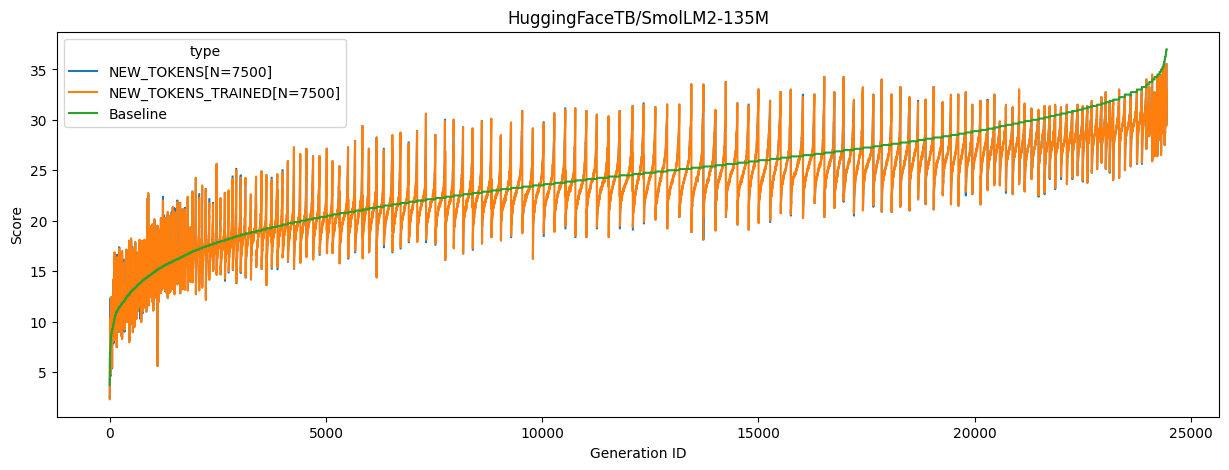
\includegraphics[width=0.75\textwidth]{Figures/rank_distribution_smolLM2.png}
    \caption[Score comparison]{Score comparison between original sub-tokens and new tokens\footnotemark}
    \label{fig:new_token_rank}
\end{figure}
\footnotetext{We ran this comparison with an additional 7500 tokens.}

\begin{figure}[H]
    \centering
    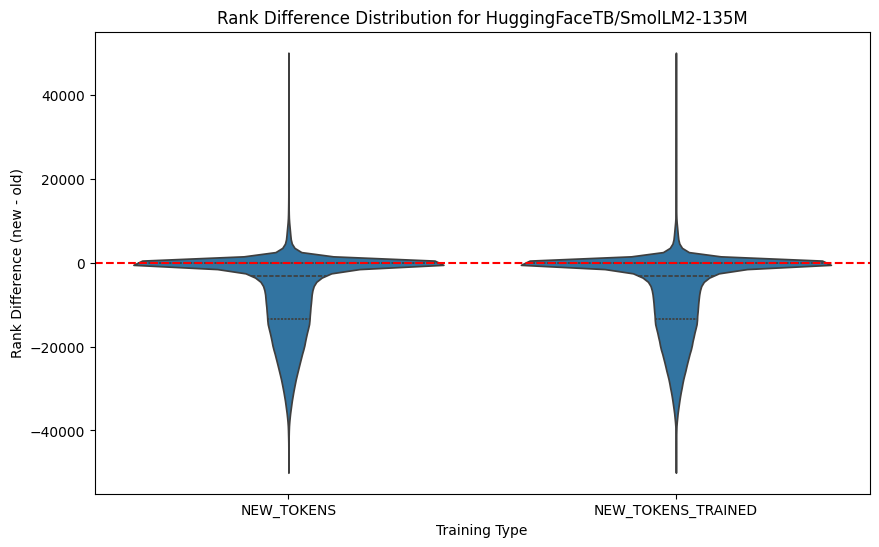
\includegraphics[width=1\textwidth]{Figures/rank_diff_dist_violin.png}
    \caption[Distribution of Rank Differences]{Distribution of rank differences across the entire results data, shown as violin plots. The x-axis indicates the training type, while the y-axis shows the rank difference $new\_token\_rank - old\_token\_rank$. Each “violin” depicts the distribution of values, where its width reflects the density of observations and the internal lines mark quartiles. 
Negative values indicate preference towards \texttt{new\_token}.}
    \label{fig:violin_rank_dist}
\end{figure}
Distribution of rank differences across the entire results data, shown as violin plots. 
The x-axis indicates the training type, while the y-axis shows the rank difference $new\_token\_rank - old\_token\_rank$. 
Each “violin” depicts the distribution of values, where its width reflects the density of observations and the internal lines mark quartiles. 
Negative values indicate preference towards \texttt{new\_token}.


The rank analysis confirms that many new tokens were indeed assigned higher probabilities than their decomposed counterparts. This indicates that models learn to prefer merged units after adaptation. Interestingly, there doesn't seem to exist a significant impact from applying further pre-training -- adding new tokens with the right initialization strategy is enough. Extended plots for additional models are presented in Appendix~\ref{annex:results-rank-comparison} (score comparison) and Appendix~\ref{annex:results-rank-differences} (rank differences).




\section{Qualitative Evaluation}
Benchmark scores and fertility metrics only partially capture the interactive experience of using a model. To complement the quantitative analysis, we conducted a qualitative comparison of completions. 
This evaluation was carried out for both European Portuguese (Table~\ref{tab:example_completions_horizontal-PT}) and English (Table~\ref{tab:example_completions_horizontal-EN}), using equivalent prompts in each language.

Generations were constrained to a maximum of 50 new tokens, which increases the likelihood of truncated phrases. Sampling was applied with the following parameters: \textit{temperature} ($0.8$), \textit{top-$p$} ($0.9$), and \textit{top-$k$} ($100$).\footnote{%
Temperature scales the logits before sampling, controlling randomness; lower values yield more deterministic generations. 
Top-$p$ (nucleus sampling) restricts choices to the smallest set of tokens whose cumulative probability exceeds $p$. 
Top-$k$ limits sampling to the $k$ most probable tokens.}





{
    % Define new commands to apply colors
    \newcommand{\prompt}[1]{\textcolor{promptcolor}{#1}}
    % \newcommand{\generation}[1]{\textcolor{generationcolor}{#1}\par}
    \newcommand{\generation}[1]{%
      {\RaggedRight\arraybackslash\color{generationcolor}\sloppy\footnotesize #1\hspace{0pt}\par}%
    }
    \begin{table}[h]
        \centering
        \begin{tabular}{p{\linewidth}}
            \toprule
            \textbf{Prompt:} \prompt{``Para calcular a raiz quadrada de um número manualmente,''} \\
            \begin{tabularx}{\hsize}{X|X|X}
            \midrule
                \textbf{Baseline} & \textbf{Adapted w/ 5000 tokens} & \textbf{Adapted and Trained} \\
                \generation{``retorna uma posição.\newline \texttt{```}python\newline x = 10\newline y = 20\newline print(f"A raiz quadrada de \{x\} e \{y\} é \{x ** ''} & \generation{``utilizando o \newline tipo de cálculo de fatorial. Por exemplo, se uma quantidade de \newline pemares a pouco mais de um alcance, seja 110000''} & \generation{``\newline e construa um número quadrado em duas partes \newline aixa e a linda, \newline A matoê estra:\newline A matoê do primeiro num méênico da raiz''} \\
            \midrule
            \end{tabularx}
            \textbf{Prompt:} \prompt{``Nos dias de hoje, democracia é o sistema politico''} \\
            \begin{tabularx}{\hsize}{X|X|X}
            \midrule
                \textbf{Baseline} & \textbf{Adapted w/ 5000 tokens} & \textbf{Adapted and Trained} \\
                \generation{``. Ao \newline demorar por 6 dias para que seja o seu emissar, a dor da elemência eleitora \newline atual aumentará e o próprio p''} & \generation{``que ele, na quais seriam \newline a diferença, de forma fatoriva, de uma média de 013020 00010000000010...''} & \generation{``, o que não se encontra nis. A que também é o democracia.\newline EIuão de Hic e da Cria de Io Paulo. \newline Hic''} \\
            \midrule
            \end{tabularx}
            \textbf{Prompt:} \prompt{``O poema seguinte contém várias palavras-chave: azul, borboleta e sol:''} \\
            \begin{tabularx}{\hsize}{X|X|X}
            \midrule
                \textbf{Baseline} & \textbf{Adapted w/ 5000 tokens} & \textbf{Adapted and Trained} \\
                \generation{``e sí, e também, e física e próximo. \newline O poema também tem como seu último último, o estudante de''} & \generation{``céu de la tierra, y vrgosos deixa. \newline Vídeo como nome: «Cicio-dei alcoba e sol», com aumos dos dcimentoimens''} & \generation{``Este estará por esqueço da esquina do lado do que a leitura seja frente ao largo do espaço”. Para outras palavras-chave,''} \\
            \bottomrule
            \end{tabularx}
        \end{tabular}
        \caption{Illustrative Examples of Model Completions (Baseline vs. Adapted vs. Adapted and Trained) for Portuguese}
        \label{tab:example_completions_horizontal-PT}
    \end{table}
}

The results reveal clear differences across conditions. Baseline generations are often syntactically incomplete, emphasizing the weak effectiveness in European Portuguese. Adapted models produce somewhat longer and more structured sentences, though improvements are modest.
Nonetheless, they frequently invent morphology or generate ungrammatical constructions. Semantic grounding remains fragile: numerical reasoning prompts yield incoherent results, while open-ended prompts (e.g., political or poetic) elicit more topically appropriate responses in the Adapted and Trained variant. 

{
    % Define new commands to apply colors
    \newcommand{\prompt}[1]{\textcolor{promptcolor}{#1}}
    \newcommand{\generation}[1]{%
      {\RaggedRight\arraybackslash\color{generationcolor}\sloppy\footnotesize #1\hspace{0pt}\par}%
    }
    \begin{table}[h]
        \centering
        \begin{tabular}{p{\linewidth}}
            \toprule
            \textbf{Prompt:} \prompt{``To calculate the square root of a number by hand,''} \\
            \begin{tabularx}{\hsize}{X|X|X}
                \midrule
                \textbf{Baseline} & \textbf{Adapted w/ 5000 tokens} & \textbf{Adapted and Trained} \\
                \generation{`` you would divide the number into equal parts and then subtract the results to get the square root of the result. In Python, we can use the built-in `sqrt()` function to calculate the square root of a number.\newline \#\#\#''} & \generation{`` the digits of the number can be marked on a piece of paper, or a digital calculator will do the job for you.\newline Step 14: Choose a suitable scale\newline Use a calculator or a digital scale to scale the numbers''} & \generation{`` the rule is to take the negative of the first digit, then multiply the result by itself, and then subtract the result\newline \#\#\# Why Square Root Calculator?\newline The square root of 1833195073330500''} \\
                \midrule
            \end{tabularx}
            \textbf{Prompt:} \prompt{``Nowadays, democracy is the political system''} \\
            \begin{tabularx}{\hsize}{X|X|X}
                \midrule
                \textbf{Baseline} & \textbf{Adapted w/ 5000 tokens} & \textbf{Adapted and Trained} \\
                \generation{`` that allows citizens to choose the leaders who will guide them in their chosen path. They are also known as the people. DEMOCRACY - The people who rule a country or an organization.DEPARTMENT''} & \generation{`` of a country or country region where the people, including elected representatives, are able to choose the leaders of the country. In other words, the people are free to govern and choose their leaders and policies for their country. In the''} & \generation{`` that allows citizens to vote for their representatives, so that they can elect a government. In a democracy, people vote for politicians to represent them. This is similar to a democracy where people elect representatives who vote for those politicians. A''} \\
            \midrule
            \end{tabularx}
            \textbf{Prompt:} \prompt{``The following poem contains several keywords: Blue, Butterfly, and Sun:''} \\
            \begin{tabularx}{\hsize}{X|X|X}
            \midrule
                \textbf{Baseline} & \textbf{Adapted w/ 5000 tokens} & \textbf{Adapted and Trained} \\
                \generation{``Here is the beginning of the poem:\newline Blue, Butterfly, and Sun\newline Blue, Butterfly, and Sun\newline Blue, Butterfly, and Sun\newline Blue, Butterfly, and Sun\newline Blue, Butterfly''} & \generation{``Blue Butterfly\newline I am blue,\newline The butterfly of my mind\newline I feel my mind\newline Throbbing in my breast,\newline And I cannot tell what to do.\newline I cannot tell what to do,''} & \generation{``Blue Butterfly\newline Blue Butterfly\newline I feel blue\newline A butterfly has flown\newline Across the blue sky\newline And I feel sad\newline I feel sad and angry\newline Ia like the butterfly''} \\
            \bottomrule
            \end{tabularx}
        \end{tabular}
        \caption{Illustrative Examples of Model Completions (Baseline vs. Adapted vs. Adapted and Trained) for English.}
        \label{tab:example_completions_horizontal-EN}
    \end{table}
}
Unsurprisingly, qualitative results mirror the quantitative findings. These results suggest that tokenizer adaptation to a new target language has no observable effect on effectiveness on the model's source language. The observed variations are attributed to sampling parameters rather than substantive changes in generation quality.

These qualitative results are presented only for the monolingual model, \texttt{SmolLM2-135M}, to better isolate the effects of adapting a model trained exclusively in one language to a different linguistic context.


\section{Limitations and Discussion}

The results reported in this chapter should be interpreted with caution. Many of the experiments rely on small-scale models such as \texttt{SmolLM2-135M}, which exhibit severe hallucination effects even before adaptation.
This constrains the extent to which improvements can be generalized. Evaluation metrics introduce further challenges: benchmark scores, while robust for task accuracy, are coarse-grained and may fail to capture subtler shifts in fluency or style, whereas fertility metrics, though informative, are sensitive to corpus size and the heuristics used for token selection.
As a result, the impact of adaptation may be underestimated in our current setup. Broader evaluations across larger architectures and human-judged fluency assessments would strengthen our findings.

Despite these caveats, the evidence points to a cautiously optimistic picture.
Vocabulary expansion does not alter benchmark accuracy, but neither does it degrade it.
Efficiency gains are substantial in small monolingual models but negligible in mid-scale multilingual ones.
Rank analyses reveal that models learn to prefer newly added tokens, suggesting an internal mechanism by which adaptation affects fluency even when benchmarks remain stable.
Qualitative analysis confirms that generations can become longer and more syntactically structured, though their semantic reliability remains weak.
Notably, source language effectiveness remains fully stable, ensuring that Portuguese adaptation does not compromise the model’s original competencies in English.

Taken together, these findings suggest that tokenizer adaptation is most promising in scenarios where baseline tokenization is inefficient and resources are limited.
For lightweight models, especially those not initially optimized for Portuguese, the benefits are concrete and measurable.
For larger multilingual systems, gains are less pronounced.
In this sense, the results confirm the central hypothesis of this dissertation: token-level interventions may provide a low-cost pathway to make English-trained models more suitable for underrepresented languages such as European Portuguese.


